\section{最大熵}
\label{sec:dsel-maxent}

一颗骰子，我们只知道长期掷出的平均点数是$4.5$，此外一无所知。若要给出一张概率表，该用哪一张？满足平均点数$4.5$的表有无穷多张。若选了一张让$6$点特别多、$1$点为零的表，就等于声称知道了“$1$点不会出现”之类平均值并未告诉我们的事。一个自然的原则是：在满足已知条件的分布中，选最不确定的那个，也就是熵最大的那个。

第~\ref{chap:information-measures}章把熵$H(Q)=-\sum_xq(x)\ln q(x)$解释为平均要问的是非题数目（以nat计）。熵越大，结果越难预测，分布中隐含的额外断言就越少。按这个标准选择分布，称为\term{最大熵原理}（maximum entropy principle）。它是一条选择规则，不是定理；定理要回答的是，按这条规则选出的分布是什么、何时存在。

\paragraph{有限支持上的最大熵}
设$\mathcal{X}$有$n$个状态，$U$是$\mathcal{X}$上的均匀分布。对$\mathcal{X}$上任意分布$Q$，
\[
 D_{\mathrm{KL}}(Q\Vert U)=\sum_xq(x)\ln\bigl(n\,q(x)\bigr)=\ln n-H(Q) .
\]
所以
\begin{equation}
 H(Q)=\ln n-D_{\mathrm{KL}}(Q\Vert U).
 \label{eq:dsel-entropy-kl-uniform}
\end{equation}
熵与“离均匀分布的KL”只差一个与$Q$无关的常数，最大化熵就是以均匀分布为参考、最小化KL。上一节的结论可以直接搬过来。

\begin{theorem}[有限支持上的最大熵分布]
\label{thm:dsel-maxent-finite}
设$\mathcal{X}$有限，$\bm{T}:\mathcal{X}\to\mathbb{R}^{k}$，$\bm{m}\in\operatorname{ri}\operatorname{conv}\{\bm{T}(x):x\in\mathcal{X}\}$。则在$\mathbb{E}_{Q}[\bm{T}]=\bm{m}$的分布中，熵的最大值由唯一的分布
\begin{equation}
 q^{*}(x)=\frac{\exp\langle\bm{\theta},\bm{T}(x)\rangle}{\sum_{y\in\mathcal{X}}\exp\langle\bm{\theta},\bm{T}(y)\rangle}
 \label{eq:dsel-maxent-finite}
\end{equation}
达到，其中$\bm{\theta}$满足$\mathbb{E}_{Q^{*}}[\bm{T}]=\bm{m}$。最大熵为
\begin{equation}
 H(Q^{*})=A_0(\bm{\theta})-\langle\bm{\theta},\bm{m}\rangle,\qquad A_0(\bm{\theta})=\ln\sum_{y\in\mathcal{X}}\mathrm{e}^{\langle\bm{\theta},\bm{T}(y)\rangle} .
 \label{eq:dsel-maxent-value}
\end{equation}
\end{theorem}

\begin{proof}
由式~\eqref{eq:dsel-entropy-kl-uniform}，问题等价于以$P=U$为参考的问题~\eqref{eq:dsel-min-kl-problem}。$U$处处为正，定理~\ref{thm:dsel-min-kl}给出唯一最优分布
\[
 q^{*}(x)=\frac1n\exp\bigl(\langle\bm{\theta},\bm{T}(x)\rangle-A(\bm{\theta})\bigr),
\]
其中
\[
 A(\bm{\theta})=\ln\frac1n\sum_y\mathrm{e}^{\langle\bm{\theta},\bm{T}(y)\rangle}=A_0(\bm{\theta})-\ln n ,
\]
代入即得式~\eqref{eq:dsel-maxent-finite}。最大熵等于$\ln n-D^{*}$，由式~\eqref{eq:dsel-min-kl-value}，
\[
 H(Q^{*})=\ln n-\langle\bm{\theta},\bm{m}\rangle+A_0(\bm{\theta})-\ln n=A_0(\bm{\theta})-\langle\bm{\theta},\bm{m}\rangle .
\]
\end{proof}

式~\eqref{eq:dsel-maxent-finite}称为\term{最大熵分布}（maximum entropy distribution）。定理中的“支持”是事先给定的：状态集合$\mathcal{X}$本身就是一条约束，不在其中的状态概率为零。若把骰子的状态集合扩大到$\{0,1,\dots,7\}$，$\ln n$和最大熵分布都会改变。在有限情形中，计数测度把每个状态看成同样重要，这是“均匀分布最不确定”的前提。

在三状态的例子中，均值$10/7$下的最大熵分布就是$(\tfrac17,\tfrac27,\tfrac47)$，熵为
\[
 H(Q^{*})=\ln7-\frac{10}{7}\ln2\approx0.9557 .
\]
约束线段的端点$(\tfrac27,0,\tfrac57)$的熵约为$0.5983$。由式~\eqref{eq:dsel-entropy-kl-uniform}与勾股恒等式，两者之差恰为$D_{\mathrm{KL}}(Q\Vert Q^{*})\approx0.3574$：熵的损失就是离最大熵分布的KL。

\paragraph{约束改变时}
回到骰子，$\mathcal{X}=\{1,\dots,6\}$，$T(x)=x$，可行矩集合是$[1,6]$。均值$m$给定后，最大熵分布是$q(x)\propto\mathrm{e}^{\theta x}$，$\theta$由
\[
 \frac{\sum_{x=1}^{6}x\,\mathrm{e}^{\theta x}}{\sum_{x=1}^{6}\mathrm{e}^{\theta x}}=m
\]
确定。它没有闭式解，用第~\ref{sec:dsel-moment-matching}节的Newton法求出。

$m=3.5$时，均匀分布本身满足约束，$\theta=0$，熵为$\ln6\approx1.792$。约束没有起作用：它排除了一些分布，但没有排除熵最大的那个。$m=4.5$时，$\theta\approx0.3710$，
\[
 Q^{*}\approx(0.0544,\ 0.0788,\ 0.1142,\ 0.1654,\ 0.2398,\ 0.3475),
\]
熵约为$1.614$。相邻点数的概率之比恒为$\mathrm{e}^{\theta}\approx1.449$，平均值的要求以最平缓的方式把质量推向大点数，没有任何一面被删去。$m=5.5$时$\theta\approx1.087$，分布约为$(0.0029,0.0086,0.0255,0.0755,0.2238,0.6637)$，熵降到约$0.953$。

再加一条约束。要求均值为$3.5$，且$\mathbb{E}_{Q}[(X-3.5)^{2}]=1$，比均匀分布的$35/12\approx2.917$小。统计量取$\bm{T}(x)=\bigl(x-3.5,\ (x-3.5)^{2}\bigr)$，由对称性第一个乘子为零，最大熵分布是$q(x)\propto\mathrm{e}^{\theta_2(x-3.5)^{2}}$，$\theta_2\approx-0.4887$：
\[
 Q^{*}\approx(0.0186,\ 0.1316,\ 0.3498,\ 0.3498,\ 0.1316,\ 0.0186),
\]
熵约为$1.417$。它是一个离散的钟形，这正是指数中出现二次项的结果。图~\ref{fig:dsel-dice-bars}画出这四张表。

\begin{BookInlineFigure}
 \centering
 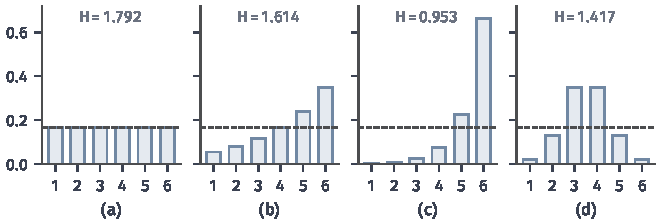
\includegraphics[width=112mm]{figures/07-probability/07-distribution-optimization/matplotlib/dsel-dice-bars/figure.pdf}
 \caption{骰子的最大熵分布（蓝色柱），深灰虚线为均匀概率$1/6$，图中标出熵（nat）。(a)$\mathbb{E}[X]=3.5$，约束不起作用。(b)$\mathbb{E}[X]=4.5$，$\theta\approx0.371$。(c)$\mathbb{E}[X]=5.5$，$\theta\approx1.087$。(d)$\mathbb{E}[X]=3.5$且$\mathbb{E}[(X-3.5)^{2}]=1$，$q\propto\mathrm{e}^{\theta_2(x-3.5)^{2}}$，$\theta_2\approx-0.489$。}
 \label{fig:dsel-dice-bars}
\end{BookInlineFigure}

增加约束只会缩小可行集合，最大熵不会增加；(d)比(a)少了约$0.375$ nat，这就是“方差为$1$”这条信息的量。最大熵还随约束值连续变化。记$H^{*}(m)$为均值为$m$时的最大熵。设$Q_1,Q_2$分别是均值$m_1,m_2$下的最大熵分布，$0\leq\lambda\leq1$，混合$\lambda Q_1+(1-\lambda)Q_2$的均值是$\lambda m_1+(1-\lambda)m_2$，由熵的凹性，
\[
 H^{*}\bigl(\lambda m_1+(1-\lambda)m_2\bigr)\geq H\bigl(\lambda Q_1+(1-\lambda)Q_2\bigr)\geq\lambda H^{*}(m_1)+(1-\lambda)H^{*}(m_2) .
\]
所以$H^{*}$是凹函数。图~\ref{fig:dsel-entropy-curve}(a)中它在$m=3.5$处取最大值$\ln6$，向两端下降，在$m=1$和$m=6$处为零，那里唯一可行的分布是单点分布；(b)中的$\theta(m)$在两端发散，与第~\ref{sec:dsel-moment-matching}节的边界情形一致。

\begin{BookInlineFigure}
 \centering
 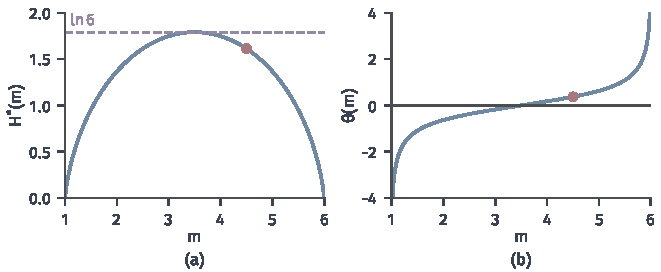
\includegraphics[width=112mm]{figures/07-probability/07-distribution-optimization/matplotlib/dsel-entropy-curve/figure.pdf}
 \caption{骰子均值为$m$时的最大熵问题。(a)最大熵$H^{*}(m)$（蓝），紫色虚线为上界$\ln6$，红点为$m=4.5$，$H^{*}\approx1.614$。(b)对应的乘子$\theta(m)$，红点为$(4.5,\,0.371)$，$m\to1$或$6$时发散。}
 \label{fig:dsel-entropy-curve}
\end{BookInlineFigure}

\paragraph{连续情形的参考测度}
对有密度的分布，第~\ref{chap:information-measures}章用微分熵$h=-\int f\ln f\,\mathrm{d}x$代替熵。这里的密度是相对于Lebesgue测度的密度，Lebesgue测度在其中扮演的角色，正是有限情形中的计数测度。一般地，设$\nu$是$\mathcal{X}$上的$\sigma$有限测度，$Q\ll\nu$，$q=\mathrm{d}Q/\mathrm{d}\nu$，在$q\lvert\ln q\rvert$对$\nu$可积时定义
\begin{equation}
 h_\nu(Q)=-\int_{\mathcal{X}}q\ln q\,\mathrm{d}\nu .
 \label{eq:dsel-entropy-reference}
\end{equation}
换一个参考测度，这个量就变成另一个泛函，最大化它得到的分布也随之不同。

看一个不带任何矩约束的例子：$\mathcal{X}=[1,\mathrm{e}]$。以$\nu=\mathrm{d}x$为参考，$\nu$的总质量是$\mathrm{e}-1$，记$R$为$[1,\mathrm{e}]$上的均匀分布，与式~\eqref{eq:dsel-entropy-kl-uniform}同样计算得
\[
 h_{\mathrm{d}x}(Q)=\ln(\mathrm{e}-1)-D_{\mathrm{KL}}(Q\Vert R),
\]
最大熵分布是均匀分布，密度$1/(\mathrm{e}-1)$。以$\nu(\mathrm{d}x)=\mathrm{d}x/x$为参考，总质量$\int_1^{\mathrm{e}}x^{-1}\,\mathrm{d}x=1$，$\nu$本身就是概率测度，
\[
 h_{\mathrm{d}x/x}(Q)=-D_{\mathrm{KL}}(Q\Vert\nu),
\]
最大熵分布是$\nu$本身，相对$\mathrm{d}x$的密度为$1/x$。换成变量$y=\ln x$，第二个参考测度就是$[0,1]$上的Lebesgue测度，它说的是“$\ln X$均匀”。两个答案的中位数分别是$(1+\mathrm{e})/2\approx1.859$与$\sqrt{\mathrm{e}}\approx1.649$，见图~\ref{fig:dsel-reference-measure}。同样是“一无所知”，用$x$计量还是用$\ln x$计量，给出不同的分布。

\begin{BookInlineFigure}
 \centering
 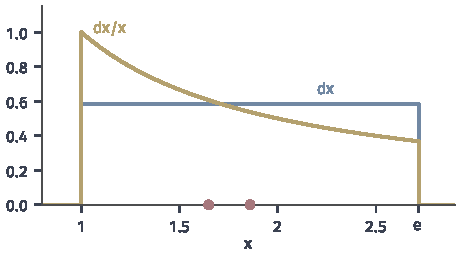
\includegraphics[width=78mm]{figures/07-probability/07-distribution-optimization/matplotlib/dsel-reference-measure/figure.pdf}
 \caption{参考测度决定最大熵分布，$\mathcal{X}=[1,\mathrm{e}]$，无矩约束。蓝：以$\mathrm{d}x$为参考，得到均匀密度$1/(\mathrm{e}-1)$；黄：以$\mathrm{d}x/x$为参考，得到密度$1/x$，即$\ln X$在$[0,1]$上均匀。两个红点是二者的中位数$\sqrt{\mathrm{e}}$与$(1+\mathrm{e})/2$。}
 \label{fig:dsel-reference-measure}
\end{BookInlineFigure}

所以在连续情形中谈最大熵，必须先说明熵是相对哪个测度计算的。有限情形中这个问题被状态集合的选择掩盖了：一旦把骰子的六面当作六个状态，计数测度就是默认的参考。

\paragraph{熵与KL的差别}
在有限情形中，最大熵与以均匀分布为参考的最小KL只差常数。一般的参考概率$P$却不能这样替换。设$P$相对$\nu$的密度$p$处处为正，$Q$相对$\nu$的密度为$q$。在$\{q>0\}$上把$\ln q$拆成$\ln(q/p)+\ln p$，乘以$q$积分，在两项都有限时得到
\begin{equation}
 h_\nu(Q)=-D_{\mathrm{KL}}(Q\Vert P)-\mathbb{E}_{Q}[\ln p] .
 \label{eq:dsel-entropy-kl-reference}
\end{equation}
第二项依赖于$Q$，所以最大化$h_\nu$与最小化$D_{\mathrm{KL}}(\cdot\Vert P)$一般选出不同的分布。负熵$-h_\nu$是“相对于$\nu$”的KL，而不是相对于某个概率分布的KL；在有限情形中两者相同，只因为$\ln p$是常数$-\ln n$。

第二项在可行集合上为常数的情形是例外。若$\ln p$是约束统计量的仿射函数，
\[
 \ln p=\langle\bm{\theta},\bm{T}\rangle-A(\bm{\theta}),
\]
则对每个满足$\mathbb{E}_{Q}[\bm{T}]=\bm{m}$的$Q$，$\mathbb{E}_{Q}[\ln p]$都等于同一个常数$\langle\bm{\theta},\bm{m}\rangle-A(\bm{\theta})$，最大熵与最小KL就重合了。下面的定理正是这样证明的。

\begin{theorem}[相对参考测度的最大熵]
\label{thm:dsel-maxent-continuous}
设$\nu$是$\mathcal{X}$上的$\sigma$有限测度，$\bm{T}:\mathcal{X}\to\mathbb{R}^{k}$可测。设$\bm{\theta}$使
\begin{equation}
 A(\bm{\theta})=\ln\int_{\mathcal{X}}\mathrm{e}^{\langle\bm{\theta},\bm{T}\rangle}\,\mathrm{d}\nu<\infty ,
 \label{eq:dsel-maxent-partition}
\end{equation}
并且相对$\nu$的密度为
\begin{equation}
 q_{\bm{\theta}}=\exp\bigl(\langle\bm{\theta},\bm{T}\rangle-A(\bm{\theta})\bigr)
 \label{eq:dsel-maxent-density}
\end{equation}
的分布$Q_{\bm{\theta}}$满足$\mathbb{E}_{Q_{\bm{\theta}}}\lVert\bm{T}\rVert_2<\infty$，$\mathbb{E}_{Q_{\bm{\theta}}}[\bm{T}]=\bm{m}$。则对每个满足$Q\ll\nu$、$q\lvert\ln q\rvert$对$\nu$可积、$\mathbb{E}_{Q}\lVert\bm{T}\rVert_2<\infty$且$\mathbb{E}_{Q}[\bm{T}]=\bm{m}$的分布$Q$，
\begin{equation}
 h_\nu(Q)=h_\nu(Q_{\bm{\theta}})-D_{\mathrm{KL}}(Q\Vert Q_{\bm{\theta}}),\qquad h_\nu(Q_{\bm{\theta}})=A(\bm{\theta})-\langle\bm{\theta},\bm{m}\rangle .
 \label{eq:dsel-maxent-identity}
\end{equation}
因此$Q_{\bm{\theta}}$是这些分布中熵最大的唯一一个。
\end{theorem}

\begin{proof}
$q_{\bm{\theta}}$处处为正，所以$Q\ll Q_{\bm{\theta}}$，密度比为$q/q_{\bm{\theta}}$。在$\{q>0\}$上，
\[
 \ln\frac{q}{q_{\bm{\theta}}}=\ln q-\langle\bm{\theta},\bm{T}\rangle+A(\bm{\theta}) .
\]
右边三项都在$Q$下可积：$\int q\lvert\ln q\rvert\,\mathrm{d}\nu<\infty$，$\bm{T}$在$Q$下可积，$A(\bm{\theta})$是常数。逐项取$Q$下的期望，
\[
 D_{\mathrm{KL}}(Q\Vert Q_{\bm{\theta}})=-h_\nu(Q)-\langle\bm{\theta},\bm{m}\rangle+A(\bm{\theta}) .
\]
对$Q=Q_{\bm{\theta}}$，由
\[
 \lvert\ln q_{\bm{\theta}}\rvert\leq\lvert\langle\bm{\theta},\bm{T}\rangle\rvert+\lvert A(\bm{\theta})\rvert
\]
知$\ln q_{\bm{\theta}}$在$Q_{\bm{\theta}}$下可积，它满足同样的条件，代入上式，左边为零，得到式~\eqref{eq:dsel-maxent-identity}的第二式。把第二式代回上式，就得到第一式。唯一性来自Gibbs不等式的等号条件。
\end{proof}

定理的形式与有限情形相同，不同之处在于两件事都要事先核对：配分积分$\int\mathrm{e}^{\langle\bm{\theta},\bm{T}\rangle}\mathrm{d}\nu$是否有限，以及候选分布的熵是否有定义。第~\ref{chap:information-measures}章已经指出，密度可以大于$1$，$-q\ln q$有正有负，正负两部分的积分都发散时熵没有意义；这样的分布不在定理比较的范围内。

\paragraph{几个连续例子}
在$\mathbb{R}$上以Lebesgue测度为参考，规定均值$\mu$与方差$\sigma^{2}$，即$\bm{T}(x)=(x,x^{2})$，$\bm{m}=(\mu,\mu^{2}+\sigma^{2})$。候选形式是$\mathrm{e}^{\theta_1x+\theta_2x^{2}}$，可积要求$\theta_2<0$，它就是高斯密度；$\mathcal{N}(\mu,\sigma^{2})$满足约束，由定理~\ref{thm:dsel-maxent-continuous}，它是给定均值与方差的密度中微分熵最大的，最大值为
\[
 h\bigl(\mathcal{N}(\mu,\sigma^{2})\bigr)=\frac12\ln(2\pi\mathrm{e}\sigma^{2}) .
\]
方差为$1$时它约为$1.419$。同样方差为$1$的Laplace密度微分熵约为$1.347$，$[-\sqrt3,\sqrt3]$上的均匀密度约为$1.242$，都更小，见图~\ref{fig:dsel-gauss-maxent}。

\begin{BookInlineFigure}
 \centering
 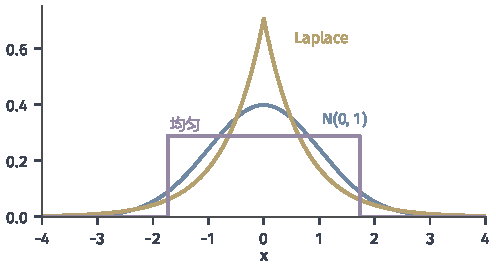
\includegraphics[width=84mm]{figures/07-probability/07-distribution-optimization/matplotlib/dsel-gauss-maxent/figure.pdf}
 \caption{均值$0$、方差$1$的三个密度。蓝：$\mathcal{N}(0,1)$，$h=\frac12\ln(2\pi\mathrm{e})\approx1.419$；黄：尺度$1/\sqrt2$的Laplace密度，$h=1+\ln\sqrt2\approx1.347$；紫：$[-\sqrt3,\sqrt3]$上的均匀密度，$h=\ln(2\sqrt3)\approx1.242$。熵相对Lebesgue测度计算，单位为nat。}
 \label{fig:dsel-gauss-maxent}
\end{BookInlineFigure}

在$(0,\infty)$上规定均值$1/\lambda$，候选$\mathrm{e}^{\theta x}$要求$\theta<0$，得到$\operatorname{Exp}(\lambda)$，最大熵为$1-\ln\lambda$。在有界区间$[a,b]$上不加任何矩约束，$\bm{T}=\bm{0}$，得到均匀分布，最大熵为$\ln(b-a)$。这三个常见分布都是“在某个支持上、给定某些矩”时的最大熵分布，支持与矩缺一不可。

最大值也可能不存在。在$\mathbb{R}$上只规定均值$\mu$，候选形式$\mathrm{e}^{\theta x}$对任何$\theta$都不可积，定理无从适用；而$\mathcal{N}(\mu,s^{2})$都满足约束，熵$\frac12\ln(2\pi\mathrm{e}s^{2})$随$s\to\infty$趋于无穷，所以上确界是$+\infty$。在$(0,\infty)$上不加约束也是如此。Lebesgue测度的总质量无穷，质量可以无限摊开，熵就没有上界。
